\documentclass[12pt, a4paper]{article}

\usepackage[utf8]{inputenc}
\usepackage[russian]{babel}
\parindent 0pt
\parskip 8pt
\usepackage{amsmath}
\usepackage{amssymb}
\usepackage{array}
\usepackage{floatrow}
\usepackage{float}
\usepackage[left=2.3cm, right=2.3cm, top=2.7cm, bottom=2.7cm, bindingoffset=0cm]{geometry} % headheight=0pt,
\usepackage{hyperref}
\usepackage{graphicx}
\usepackage{multicol}
\usepackage{fancyhdr} 
\usepackage{extramarks}
\usepackage[usenames,dvipsnames]{color}
\usepackage{titlesec}
\usepackage{tikz}
\definecolor{grey}{RGB}{128,128,128}

\pagestyle{fancy}
\fancyhf{}
\lhead{Билет № 2.5}
\chead{Суперскалярная и VLIW архитектуры}
\rhead{\thepage}
\lfoot{made with Ы}
\cfoot{}
\rfoot{\today}
\renewcommand\headrulewidth{0.4pt}
\renewcommand\footrulewidth{0.4pt}

\titlespacing*{\section}{0pt}{5pt}{0pt}
\titlespacing*{\subsection}{0pt}{5pt}{0pt}
\titlespacing*{\subsubsection}{0pt}{5pt}{0pt}

\begin{document}
Конвеер это очень хорошо, но хочется ещё быстрее. Как это сделать? Сделать много конвееров.
\section{VLIW}
\textbf{VLIW} - Very Long Instruction Word. Просто взяли и сделали несколько конвееров (не обязательно одинаковых, например, стадия обращения к памяти может быть только у одного конвеера или только некоторые конвееры могут уметь делить).\\
Почему эта штука называется VLIW - потому что у неё очень длинные инструкции(вот это поворот).
\begin{figure}[h]
    \centering
    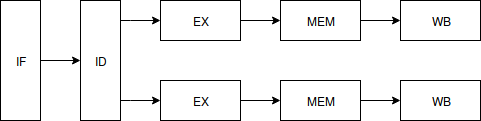
\includegraphics[width=0.8\linewidth]{images/VLIW.png}
    \caption{VLIW}
    \label{fig:VLIW}
\end{figure}
\subsection{Преимущества}
\begin{itemize}
    \item Простое железо
    \item У компилятора больше ресурсов (времени и памяти), чем у планировщика в superscalar. Вроде как можем попробовать лучше соптимизировать код под конвееры. 
\end{itemize}
\subsection{Недостатки}
\begin{itemize}
    \item Сложно написать хороший компилятор
    \item Любое изменение микроархитектуры ведет к изменению ISA. Т.е. если добавили конвеер, то чтобы он использовался, код надо как минимум перекомпилировать. Если убрали конвеер, то чтобы код вообще работал надо перекомпилировать.
    \item Из-за того, что инструкции сложно кодируются, стадия ID очень сложная. 
\end{itemize}
\subsection{Примеры}
Эльбрус (ещё советский компьютер)
\section{Superscalar}
\textbf{Superscalar} - теперь взяли и добавили умную железку \textit{Sheduler}. Теперь эта железка распределяет, какую команду куда отправить.
\begin{figure}
    \centering
    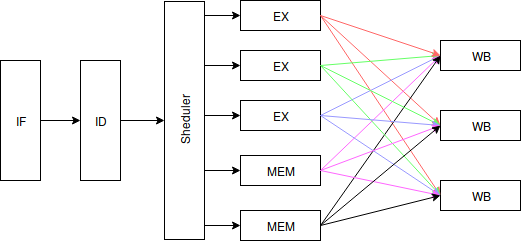
\includegraphics[width=0.8\linewidth]{images/Superscalar.png}
    \caption{Superscaalr}
    \label{fig:Superscalar}
\end{figure}
\subsection{Отчаявшийся планировщик}
Планировщики бывают умными и не очень. Самый простой планировщик берет первую команду, кидает её на конвеер. Смотрит на следующую команду: если она независима от первой, он кидает её на конвеер. Если зависима, то \textit{планировщик отчаивается} и ждет выполнения первой команды.\\
Если же планировщик умный, то он умеет искать в своей очереди команд независимые.\\
Рассмотрим планировщики начиная от менее интеллектуальных.
\subsubsection{InO/InO}
\textbf{In Order/In Order.} Команды выполняются ровно в том порядке, в каком они поступили в очередь планировщика. Пока все предыдущие команды не исполнятся, новые не поступят на конвеер. Преимущества такого подхода: достаточно простая железка, только RaW хазард. Недостатки: недостаточно быстро.
\subsubsection{Ino/OoO}
\textbf{In Order/Out of Order.} Команды поступают на выполнение в том порядке, в каком они поступили в очередь планировщика, но заканчивают исполняться не обязательно в этом же порядке.\\
Пример:\\
MUL R1 R2 R3\\
ADD R4 R2 R3\\
SUB R1 R4 R5\\
Сначала на исполнение отправляются команды MUL и ADD (они независимые). ADD завершает исполнение первым, на конвеер поступает команда SUB. Она пишет значение в R1. Потом завершает выполнение команда MUL и пишет в R1 свой результат. В итоге, по окончанию выполнения программы: в R1 должно было лежать $R4 - R5$, а лежит $R2 * R3$.\\
Такой конфликт называется \textbf{WaW} (Write after Write).
\subsubsection{OoO/OoO}
\textbf{Out of Order/Out of Order.} Команды поступают на выполнение в порядке, который устанавливает планировщик.\\
Тут так же бывает RaW и WaW хазарды. Но кроме них случается ещё и \textbf{WaR} (Write after Read) хазард.\\
Пример WaR:
MUL R1 R2 R3\\
XOR R6 R1 R5\\
ADD R4 R2 R3\\
SUB R5 R4 R5\\
Сначала начнет выполнятся MUL и ADD. Затем ADD закончит выполнение, на конвеер пойдёт SUB. Затем закончит выполнение MUL. Начнет выполняться XOR и возьмет уже измененное SUB значение. ОЖВП.\\
Пример WaW:
MUL R1 R2 R3\\
XOR R6 R1 R5\\
ADD R4 R2 R3\\
SUB R1 R4 R5\\
DIV R7 R1 R0\\
Сначала начнут выполняться MUL и ADD. Затем ADD выполнится, выполнится SUB. Затем MUL закончит выполнение, начнет выполняться XOR. Он правильно возьмёт значение R1 у MUL, но в конце в R1 окажется не то, что должно было логически. Т.е. в R1 кажется результат выполнения XOR, а не SUB.
\subsection{О хазардах}
RaW принципиально отличается от WaW и WaR. RaW - конфликт логической зависимости команд, он появляется тогда, когда какой-то из команд требуется значение предыдущей. WaR и RaW - конфликты "технические", возникающие из-за недостатка регистра.\\
WaR и RaW необходимо решать. Но просто добавить регистров нельзя (изменять ISA достоаточно больно). Поэтому такие хазарды решаются аппаратно с помощью переименования регистров. Т.е. аппаратных регистров существует больше, чем логических (видимых программно).\\
Такие конфликты решает планировщик с помощью внутренней таблицы сопоставлений программных и аппаратных регистров.\\
Кроме того, в решении конфликтов участвует еще и стадия WB. Следовательно она сложная, следовательно WB стадий меньше, чем конвееров. Планировщик никогда не запустит команды так, чтобы одновременно на стадию WB отправилось больше команд, чем есть блоков WB.
\subsection{Преимущества}
\begin{itemize}
    \item Проще писать компилятор
    \item Планировщик знает про систему сильно больше, чем компилятор. Например, если случился кэш-промах, то планировщик может знать об этом, знать, что ничего связанного с этой командой обращения к памяти ему в ближайшие 200 тактов не светит и оптимизировать работу исходя из этого знания. 
    \item Код компактнее и лучше кэшируется. Т.к. NOP не нужно прописывать программисту/компилятору, процессор сам разберется -> не храним NOP в коде, значит храним в кэше более полезные инструкции.
    \item Можем спокойно менять внутреннее устройство (количество конвееров и то, что каждый из них умеет), не затрагивая ISA.
\end{itemize}
\subsubsection{Недостатки}
\begin{itemize}
    \item Чем умнее планировщик, тем дороже железка.
    \item Сложная стадия WB: она занимается не только записью в регистры, но и синхронизацией.
\end{itemize}
\subsection{Примеры}
x86 - новые почти все OoO/OoO, Атомы - InO/*, Pentium I InO/InO.\\
ARM - помощнее OoO/OoO, поэнергоэффективнее InO/InO.
\end{document}